\begin{figure}[t]
\centering
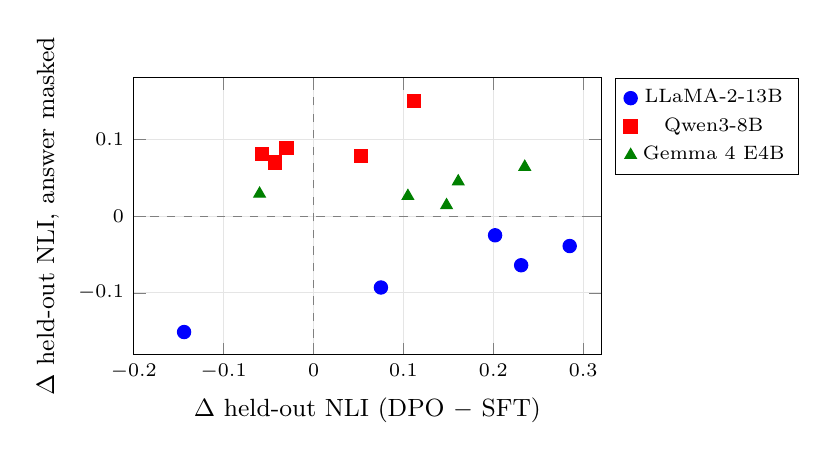
\begin{tikzpicture}
\begin{axis}[width=0.62\linewidth,height=0.42\linewidth,
  xlabel={$\Delta$ held-out NLI (DPO $-$ SFT)}, ylabel={$\Delta$ held-out NLI, answer masked},
  xmin=-0.2,xmax=0.32,ymin=-0.18,ymax=0.18, grid=major, grid style={gray!20},
  legend pos=outer north east, legend style={font=\scriptsize}, tick label style={font=\scriptsize}, label style={font=\small}]
\addplot[black!50,dashed,forget plot] coordinates {(-0.2,0) (0.32,0)};
\addplot[black!50,dashed,forget plot] coordinates {(0,-0.18) (0,0.18)};
\addplot[only marks,mark=*,mark size=2.4pt,color=blue] coordinates {(0.075,-0.093) (0.285,-0.039) (-0.144,-0.151) (0.202,-0.025) (0.231,-0.064)};
\addlegendentry{LLaMA-2-13B}
\addplot[only marks,mark=square*,mark size=2.4pt,color=red] coordinates {(-0.043,0.070) (-0.030,0.089) (0.112,0.150) (-0.057,0.081) (0.053,0.078)};
\addlegendentry{Qwen3-8B}
\addplot[only marks,mark=triangle*,mark size=2.4pt,color=green!50!black] coordinates {(0.161,0.045) (-0.060,0.029) (0.105,0.026) (0.235,0.064) (0.148,0.014)};
\addlegendentry{Gemma~4 E4B}
\end{axis}
\end{tikzpicture}
\caption{Where the entailment gain comes from. Each point is one (model, test set) cell of Table~\ref{tab:main}. $x$: change in held-out NLI after DPO. $y$: the same change after the correct answer's key terms are masked in the explanation. LLaMA-2 cells (blue) gain on $x$ but fall below zero on $y$: the gain is restating the answer. Gemma~4 cells (green) stay above zero on $y$ while their outputs get shorter. Qwen3 (red) rises on $y$ but its outputs triple in length (Table~\ref{tab:main}).}
\label{fig:masking}
\end{figure}
